\section{On-demand Producer Service}\label{sec:OnDemandProducer}\index{on demand producer}
\subsection{Description}

On-demand Producer resources are created by the On-demand Producer Service
at the request of a user who wishes to make an external data store available
through a virtual database. They are registered in the same way as the other
producer types and their queries are parsed, validated and authorized like
queries to the other producer types, but they only support static queries,
are not used by Secondary Producers, have no internal tuple storage, and
have no concept of retention periods. As the picture below shows, queries are
simply handed off to a user-defined application (\textit{query handler}) that
is expected to process the query and return the resulting tuples on demand.

\begin{center}
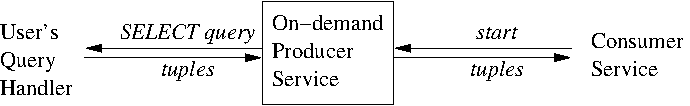
\includegraphics[width=110mm]{odp_detail}
\end{center}

The On-demand Producer Service is responsible for authenticating all users and
services that connect to it and for authorizing all operations and requests to
access its users' external data stores, as specified in chapter
\ref{sec:Security}.

\subsection{Interface}

\subsubsection{User Interface}

\begin{method}{createOnDemandProducer}
\inpar{xsd:string hostName}{Hostname of machine to which to connect to get data
to answer queries.}
\inpar{xsd:int port}{Port to which to connect to get data
to answer queries.}
\outhead{Tuple(1..1)}{}
\outpar{xsd:int connectionId}{connectionId of new On-demand Producer resource.} 
\desc
Creates a new On-demand Producer resource and returns its endpoint. The
On-demand Producer is not added to a Registry until \textit{declareTable} is
called. On-demand producers have no tuple stores and only support static
queries.
\end{method}


\begin{method}{declareTable}
\inpar{xsd:int connectionId}{On-demand Producer resource identifier.}
\inpar{xsd:string tableName}{VDBTable to register.}
\inpar{xsd:string predicate}{Producer's predicate.}
\OK
\desc
Adds a table to the list of tables for which this producer will return tuples,
as described in \ref{sec:OnDemandProducerDeclaring}.
The table name must have an explicit virtual database name prefix (separated
from it by a dot). The format of the predicate is specified
in \ref{sec:SQLPredicates}; all returned tuples must match this predicate or
they will be rejected by the producer. 
\end{method}

See also the common producer service operations:
getHistoryRetentionperiod~\ref{op:getHistoryRetentionPeriod}.

See also the common resource management service operations:
close~\ref{op:close} and
destroy~\ref{op:destroy}.

See also the operations common to all services:
getProperty~\ref{op:getProperty}.

\subsubsection{System Interface}

See  the common producer service operations:
start~\ref{op:start} and abort~\ref{op:producerabort}.

See the common resource management service operation:
ping~\ref{op:resourceping}.

\subsection{Details}
\subsubsection{Creating and destroying On-demand Producers}\label{sec:OnDemandProducerCreating}

A new on-demand producer resource is created when a user calls the
\textit{createOnDemandProducer} operation and is destroyed when the
user calls the \textit{close} or \textit{destroy} operations. In
addition, if the service does not hear from the user for a period
exceeding the \textit{termination interval}, the service will initiate
a \textit{close} operation on the resource. A call to any user
operation on the resource is sufficient to keep it alive.

\subsubsection{The query handler}

The on-demand producer connects to the specifed hostname and port via an SSL
socket connection to answer user queries. R-GMA
expects the query handler application to be listening for queries
throughout the lifetime of the on-demand producer resource.

\subsubsection{Declaring tables}\label{sec:OnDemandProducerDeclaring}

On-demand producers must register any tables for which they will
answer queries by calling \textit{declareTable}. The On-demand
Producer Service registers the producer as a publisher for that table
by calling the registry's \textit{registerProducerTable} operation and
will periodically re-send the \textit{registerProducerTable} to the
registry on the user's behalf, to maintain the producer's entries in
the registry throughout its lifetime. The user can declare more than
one table in a single producer, and these can even be in different
virtual databases. Whether or not ``join'' queries can be processed
depends only on the capabilities of the query handler that answers the
producer's queries.

\subsubsection{Processing Queries}\label{sec:OnDemandProducerQueryProcessing}

Consumer Services send a \textit{start} message to an On-demand
Producer to request it to execute a query and start streaming the
resulting tuples back to the consumer service. The query is forwarded
to the registered query handler for processing (see below for the protocol),
and the tuples (if any)
returned by the query handler are streamed by the On-demand Producer service
back to the consumer's streaming server, exactly as in a one-time query to
any other type of producer (see \ref{sec:ConsumerStreaming}). A query may be
stopped by the consumer service by calling \textit{abort}. Queries
will also be automatically aborted by the On-demand Producer Service
if they run for more than the \textit{timeout} specified in the call
to \textit{start}.

The On-demand producer service will append the standard metadata columns
(see \ref{sec:PrimaryProducerInserting}) to each tuple for
consistency with the table definition in the schema, before streaming
them back to the consumer service, but the columns will all be populated
with NULLs.

See section
\ref{sec:SQLCharacterSets} for information about the character sets used in
R-GMA (this will affect both the SQL query sent to the query handler, and its
response).

\subsubsection{Query handler protocol}

The On-demand Producer service contacts the query handler by opening a TCP
connection on the host
and port specified in the URI and writing the SQL SELECT query and the maximum
number of tuples it will allow in a result set, to the port. The two parameters
are separated by a semi-colon and the request is terminated by a CR-NL end of 
line marker. The query handler must respond by sending a series of result sets
(chunks) each containing no more than the requested number of tuples, or it must
return an exception. The query handler should mark the end of the response by
shutting the TCP connection.

The result sets and exceptions returned by the query handler are XML fragments,
each containing a single XMLResultSet or XMLException. The XMLResultSet looks
like this:

\begin{verbatim}
<?xml version="1.0" encoding="UTF-8" standalone="no"?>
  <XMLResultSet endOfResults="true">
    <columnMetaData>
      <name>column-name</name>
      <type>NNN</type>
      <table>table-name</table>
    </columnMetaData>
    <row>
      <col>column-value</col>
      <col isNull="true"/>
    </row>
  </XMLResultSet>
\end{verbatim}
                                                                                
where \textit{columnMetaData} and \textit{col} are repeated for each
column, and \textit{row} is repeated for each row. The valid values
for \textit{type} are 4 (INTEGER), 7 (REAL), 8 (DOUBLE PRECISION), 91
(DATE), 92 (TIME), 93 (TIMESTAMP), 1 (CHAR) and 12 (VARCHAR). The
\textit{endOfResults} and \textit{isNull} flags both default to \textit{false} if
omitted. The \textit{XMLResultSet} element is allowed to be entirely
empty.  The last result set must contain an \textit{endOfResults} flag
set to \textit{true} (even if it is empty).

The XMLException looks like this:

\begin{verbatim}
<?xml version="1.0" encoding="UTF-8" standalone="no"?>
  <XMLException>
    <message>message-string</message>
  <XMLException>
\end{verbatim}

The On-demand producer service will shut the TCP connection if the query
handler exceeds the tuple limit in a single result set (chunk), or
it receives an \textit{abort} request, or if some other error occurs. The
query handler must ensure that the result of a query does not change during
the time it takes to deliver all of the tuples to the on-demand producer
service.

\subsection{Error Handling}

The default handling for all errors is to stop processing, make the resource
stable if possible and notify the user
(see section \ref{sec:BackgroundErrorReporting}).
